\documentclass[a4paper,12pt]{report}

\usepackage{efbox,graphicx}


\usepackage[a4paper, bindingoffset =0.3in, left=1in,right=1in,top=1in,bottom=1in,footskip=0.25in]{geometry}

\usepackage{caption}

\usepackage{times}
\usepackage{array}
\newcolumntype{C}[1]{>{\centering\arraybackslash}p{#1}}
\usepackage{siunitx,booktabs,threeparttable,caption}

\sisetup{separate-uncertainty=true}
\usepackage{nomencl}
%\usepackage{fancyhdr}
\usepackage[T1]{fontenc}
\usepackage{setspace}
\usepackage{amsmath}
%\usepackage{algorithm}
%\usepackage{algpseudocode}
\usepackage{array}
\usepackage{mdwmath}
\usepackage{eqparbox}
\usepackage{amsmath}
\usepackage{mathtools}
\usepackage{natbib}
\usepackage{float}
\usepackage{lmodern}
\usepackage{mathrsfs}
\usepackage{enumitem}
\usepackage{multirow,multicol}
\usepackage[labelfont=bf]{caption}
\usepackage{amsfonts}
\usepackage{amssymb}
\usepackage{amsbsy}
\usepackage{url}
\usepackage{xurl} % [FIX] Breaks long URLs across lines in references
\usepackage{ifthen} % [FIX] Required for the \ifthenelse macro at the bottom of the file
\usepackage{verbatim}
\usepackage{bbm}
\usepackage{makeidx}
\usepackage{latexsym}
\usepackage{euscript}
\usepackage{lastpage}
\usepackage{geometry}
\usepackage[pagestyles]{titlesec}
\newcolumntype{L}[1]{>{\raggedright\arraybackslash}p{#1}}
\usepackage{tabularx}
\usepackage{stackengine}
\usepackage{pgfplots}
\usepackage{tikz}
\pgfplotsset{width=15cm,compat=newest}
\definecolor{findOptimalPartition}{HTML}{D7191C}
\definecolor{storeClusterComponent}{HTML}{FDAE61}
\definecolor{dbscan}{HTML}{ABDDA4}
\definecolor{constructCluster}{HTML}{2B83BA}
\usepackage{lastpage}
\usepackage{fancyhdr}
%\pagestyle{fancy} 
\usepackage{pdfpages}
\usepackage{adjustbox}

%\usepackage{pdftexcmds}
%%%%%%%%%%%%%%%%%%%%%%%%%%%%%%%%%%%%%
%\usepackage{subcaption}
\usepackage{subfigure}
\usepackage{longtable}
\usepackage{rotating}
\usepackage{lscape}
\usepackage[normalem]{ulem}
\useunder{\uline}{\ul}{}
\usepackage{lscape}
\usepackage{longtable}
\usepackage{algcompatible}
\usepackage{graphicx}
%\usepackage{caption}
%\usepackage{subcaption}

\newcommand{\hd}{\rotatebox{90}}
\usepackage[linesnumbered,ruled,vlined]{algorithm2e}
\SetKwInput{KwInput}{Input}                % Set the Input
\SetKwInput{KwOutput}{Output}              % set the Output
\SetKwInput{KwResult}{Outcome}              % set the Output
\usepackage{color, colortbl}
\usepackage{textcomp}
\usetikzlibrary{fit, backgrounds, matrix, arrows.meta}
\usepackage{framed}
\efboxsetup{linecolor=black,linewidth=0.75pt}
\renewcommand{\headrulewidth}{0pt}
\renewcommand{\footrulewidth}{0pt}
\usepackage{wrapfig}
\usepackage{siunitx}
%%%%%%%%%%%%%%%%%%%%%%%%%%%%%%%%%%%%%%%%%%%%%%%%%%%%%%%%%%%%%%%%
\renewcommand{\baselinestretch}{1.3}
%\renewcommand\thesection{\arabic{section}}
\captionsetup[table]{justification=raggedright,singlelinecheck=off}
%\newpagestyle{main}{\setfoot{}{}{Page \textbf{\thepage} of \textbf{\pageref{LastPage}}}}
%\pagestyle{main}

\renewcommand\bibname{\Large References}
% [FIX] Commented out until figures are added to avoid the "Unused \captionsetup[figure]" warning
% \captionsetup[figure]{labelfont={bf},labelformat={default},labelsep=period,name={Fig.}}
\captionsetup[table]{labelfont={bf},labelformat={default},labelsep=space,name={Table}}
%\bibliographystyle{unsrt}
%\bibliographystyle{apalike}
\bibliographystyle{abbrvnat}
\setcitestyle{authoryear,open={(},close={)}}
%\bibliographystyle{abbrvnat}

% [FIX] Suppress harmless badbox warnings
\hfuzz=2pt
\hbadness=10000
\emergencystretch=2em

%%%%%%%%%%%%%%%%%%%%%%%%%%%%%%%%%%%%%%%%%%%%%%%%%%%%%%%%%%%%%%%%%%%%%%%%%%%%%%%%%%%%%%
\begin{document}
%! TEX root = ../main.tex
\begin{titlepage}
    \centering
    
    % Project Title
    \vspace*{0.1cm}
    {\fontsize{16}{20}\selectfont\textbf{Development of Autonomous Mobile Robot with\\ Natural Language Processing and Operational Dashboard}\par}
    
    \vspace{0.4cm}
    {\fontsize{9}{15}\selectfont\textbf{A Project Report Submitted in Partial Fulfillment of the Requirements for the Degree of}\par}
    
    \vspace{0.5cm}
    {\fontsize{16}{15}\selectfont\textbf{Bachelor of Technology in Robotics and Automation}\par}
    
    \vspace{0.5cm}
    {\fontsize{12}{15}\selectfont\textbf{By}\par}
    
    \vspace{0.2cm}
    {\fontsize{13}{15}\selectfont\textbf{Aditya Roy (23070127004)}\par}
    {\fontsize{13}{15}\selectfont\textbf{Palash Modi (23070127041)}\par}
    {\fontsize{13}{15}\selectfont\textbf{Sanvi Pathare (23070127053)}\par}
    {\fontsize{13}{15}\selectfont\textbf{Gaurab Kushwaha (23070126045)}\par}
    {\fontsize{13}{15}\selectfont\textbf{Anjal Poudel (23070126171)}\par}
    
    % University Logo
    \vspace{0.8cm}
    
\includegraphics[scale=0.12]{Misc/Symbiosis-Logo}\par
    
    % Guide Details
    \vspace{0.8cm}
    {\fontsize{12}{15}\selectfont\textbf{Under the Guidance of}\par}
    
    \vspace{0.3cm}
    {\fontsize{13}{15}\selectfont\textbf{Dr. Aniket Nargundkar}\par}
    {\fontsize{12}{14}\selectfont Assistant Professor,\par}
    \vspace{0.2cm}
    {\fontsize{13}{15}\selectfont\textbf{Dr. Shivali Wagle}\par}
    {\fontsize{12}{14}\selectfont Associate Professor,\par}
    {\fontsize{12}{14}\selectfont Symbiosis Institute of Technology, Pune\par}
    
    % University Name
    \vspace{0.8cm}
    {\fontsize{12}{15}\selectfont\textbf{Department of Robotics and Automation}\par}
    {\fontsize{12}{15}\selectfont\textbf{SYMBIOSIS INSTITUTE OF TECHNOLOGY}\par}
    {\fontsize{11}{14}\selectfont\textbf{A Constituent of Symbiosis International (Deemed University), Pune--412115}\par}
    
    % Year
    \vspace{0.3cm}
    {\normalsize\textbf{2026-27}\par}
    
\end{titlepage}
\thispagestyle{empty}
\newpage
\pagenumbering{roman} % Roman numbering for front matter
\setcounter{page}{1}
\newpage
\thispagestyle{plain}

\begin{center}
    {\fontsize{16}{20}\selectfont\textbf{Endorsement of Project Work}}\\[1.2cm]
\end{center}

\vspace{0.5cm}

\noindent
This is to certify that the project report titled 
\textbf{``Development of Autonomous Mobile Robot with Natural Language Processing and Operational Dashboard''} has been prepared in the prescribed format 
and carried out satisfactorily by the student group. 
The work is deemed appropriate to be presented during the 
\textbf{Second Review of the B.Tech Project}.

\vspace{1.5cm}

\noindent
\textbf{Place:} Pune \hfill \textbf{Date:} 15th September 2026 

\vspace{1.5cm}

\renewcommand{\arraystretch}{2.0} % increase row height
\begin{center}
\begin{tabular}{p{7cm} p{7cm}}
    \multicolumn{1}{c}{\textbf{Students Name and Signature}} & 
    \multicolumn{1}{c}{\textbf{Guide Name}} \\[1cm]

    \multicolumn{1}{c}{\parbox{7cm}{\centering \rule{6cm}{0.3pt} \\ Aditya Roy (23070127004)}} &
    \multicolumn{1}{c}{\parbox{7cm}{\centering \rule{6cm}{0.3pt} \\ Dr. Aniket Nargundkar}} \\[1cm]

    \multicolumn{1}{c}{\parbox{7cm}{\centering \rule{6cm}{0.3pt} \\ Palash Modi (23070127041)}} &
    \multicolumn{1}{c}{\parbox{7cm}{\centering \rule{6cm}{0.3pt} \\ Dr. Shivali Wagle }} \\[1cm]

    \multicolumn{1}{c}{\parbox{7cm}{\centering \rule{6cm}{0.3pt} \\ Sanvi Pathare (23070127053)}} &
    \multicolumn{1}{c}{} \\[1cm]

    \multicolumn{1}{c}{\parbox{7cm}{\centering \rule{6cm}{0.3pt} \\ Gaurab Kushwaha (23070126045)}} &
    \multicolumn{1}{c}{} \\[1cm]

    \multicolumn{1}{c}{\parbox{7cm}{\centering \rule{6cm}{0.3pt} \\ Anjal Poudel (23070126171)}} &
    \multicolumn{1}{c}{} \\
\end{tabular}
\end{center}

\vspace{2cm}

\vspace{2cm}



\thispagestyle{plain}
%\setcounter{page}{1}
%\pagenumbering{roman}
%\include{Front/3_Abstract}
%\setcounter{page}{4}
%\include{Front/4_Acknowledgment}
%\setcounter{page}{5}
%\addtocontents{toc}{\protect\thispagestyle{plain}}
%\addtocontents{toc}{\protect\thispagestyle{plain}}
\tableofcontents
\thispagestyle{plain}
%\setcounter{page}{2}

\newpage
\listoffigures
\thispagestyle{plain}
\newpage
\listoftables
\thispagestyle{plain}
\newpage
%\input{Front/5_Listofsym}
%\thispagestyle{empty}
%%%%%%%%%%%%%%%%%%%%%%%%%%%%%%%%%%%%%%%%%%%%%%%%%%%%%%%%%%%%%%%%%%%%%%%%%%%%%%%%%%%%%%
\newpage
\setcounter{page}{1}
\pagenumbering{arabic}
%%%%%%%%%%%%%%%%%%%%%%%%%%%%%%%%%%%%%%%%%%%%%%%%%%%%%%%%%%%%%%%%%%%%%%%%%%%%%%%%%%%%%%%
\pagestyle{plain}
%! TEX root = ../main.tex
\chapter{Introduction}
\label{chap:introduction}

Modern industrial environments, laboratories, and warehouses increasingly deploy Autonomous Mobile Robots (AMRs) for automated material transport and site monitoring \cite{macenski2021slam}. Unlike conventional Automated Guided Vehicles (AGVs) that depend on physical tracks or magnetic tape, AMRs leverage Simultaneous Localization and Mapping (SLAM) to perceive their surroundings and navigate around dynamic obstacles \cite{thrun2005probabilistic}. However, configuring and dispatching these systems typically demands specialized engineering skills, terminal commands, or rigid proprietary software.

This project addresses these challenges by integrating Natural Language Understanding (NLU) with edge-computed navigation and cloud operational telemetry. An integrated Large Language Model (LLM) processing engine parses plain text commands into spatial coordinates, while a lightweight MQTT/HTTP pipeline streams hardware diagnostics to a centralized Power BI dashboard running on a single-board computer architecture.

\section{Background}
Industrial material transport is shifting from fixed-path AGVs to agile, infrastructure-free AMRs~\citep{siegwart2011introduction}.
Furthermore, critical runtime metrics—such as wheel velocities, motor PWM levels, battery state of charge (SoC), and sensor health—are often restricted to onboard operating system logs or desktop visualization tools like RViz \cite{openrobotics2024nav2}. Bridging natural language processing with cloud-based business intelligence dashboards provides an intuitive operational interface and centralized supervisory tracking.

\section{Motivation}
This study focuses on two operational objectives:
\begin{itemize}
    \item \textbf{Democratizing Robot Control:} Allowing non-technical staff to issue natural language mission directives (e.g., ``Go to Charging Station 2''), which the system translates into navigation waypoints \cite{brown2020language, openai2024gpt}.
    \item \textbf{Operational Transparency:} Streaming battery voltage, localization coordinates, and motor health via low-overhead telemetry protocols to a cloud dashboard for real-time monitoring \cite{oasis2019mqtt, microsoft2024powerbi}.
\end{itemize}

\section{Recent Trends}
This work builds on three converging technologies:
\begin{itemize}
    \item \textbf{LLM-Driven Semantic Navigation:} Moving from rigid keyword parsing to transformer models capable of contextual spatial reasoning \cite{brown2020language, openai2024gpt}.
    \item \textbf{Cloud-Connected Telemetry Dashboards:} Transitioning local visualization to cloud-hosted business intelligence suites via lightweight protocols \cite{oasis2019mqtt, microsoft2024powerbi}.
    \item \textbf{Edge Computing on Accessible Single-Board Hardware:} Deploying 2D SLAM, dynamic path planning, and API dispatching concurrently on embedded hardware \cite{siegwart2011introduction}.
\end{itemize}

\section{Significance of the Study}
This project demonstrates that 2D LiDAR SLAM, dynamic obstacle avoidance, and cloud-assisted LLM command interpretation can be deployed reliably on embedded edge hardware without requiring industrial compute units \cite{thrun2005probabilistic, macenski2021slam, openrobotics2024nav2}. % 1.Introduction
%! TEX root = ../main.tex
\chapter{Review of Relevant Literature}
\label{ch:literature_review}

The deployment of Autonomous Mobile Robots (AMRs) in industrial, warehousing, and service contexts integrates probabilistic state estimation, real-time path planning, distributed Internet of Things (IoT) telemetry, and Human-Robot Interaction (HRI). This chapter synthesizes existing research across these four foundational domains, analyzes state-of-the-art implementations, and identifies the technical gaps addressed by this work.

\section{Simultaneous Localization and Mapping (SLAM)}
Simultaneous Localization and Mapping constitutes the core capability required for autonomous platform navigation in uncharted or dynamic spaces. The theoretical foundations of probabilistic SLAM were formalized by \citet{thrun2005probabilistic}, establishing that robot pose and environmental map features must be modeled as joint probability distributions over time. 

Early solutions relied heavily on Extended Kalman Filters (EKF) and particle filters, as surveyed by \citet{bailey2006slam1,bailey2006slam2}. While EKF-SLAM linearizes non-linear kinematic motion models, its computational complexity scales quadratically as $\mathcal{O}(N^2)$ with the landmark count $N$, rendering it inefficient for large-scale indoor environments. Particle-filter approaches such as Rao-Blackwellized particle filtering decoupled map generation from pose tracking, yet remained vulnerable to particle depletion in sprawling geometric loops.

Recent industrial implementations have largely pivoted to 2D LiDAR graph-based SLAM architectures. \citet{macenski2021slam} developed \textit{SLAM Toolbox}, a graph-optimization framework built specifically for ROS~2. SLAM Toolbox employs scan matching via the Ceres non-linear optimization solver and maintains an active pose graph that supports dynamic relocalization, multi-session map merging, and lifelong mapping. Operating on planar 2D LiDAR range data, it generates high-fidelity 2D occupancy grid maps with substantially reduced compute overhead compared to 3D point-cloud SLAM, making it well suited for edge single-board computers (SBCs).

\section{Autonomous Navigation and Kinematic Motion Control}
Once an environment is mapped, autonomous navigation requires resolving the mathematical relationship between actuator velocities and vehicle trajectories.

\subsection{Differential Drive Kinematics}
The differential drive platform is widely favored for indoor mobile robots due to its mechanical simplicity and zero-radius turning capability~\citep{siegwart2011introduction}. The forward kinematic model defines linear velocity $v(t)$ and angular velocity $\omega(t)$ in the robot frame as a function of wheel angular velocities ($\dot{\phi}_L$, $\dot{\phi}_R$), wheel radius $r$, and track gauge $b$:
\begin{equation}
    v(t) = \frac{r}{2} \left( \dot{\phi}_R(t) + \dot{\phi}_L(t) \right)
\end{equation}
\begin{equation}
    \omega(t) = \frac{r}{b} \left( \dot{\phi}_R(t) - \dot{\phi}_L(t) \right)
\end{equation}

Integrating these velocities across time yields Dead Reckoning odometry. However, real-world implementations suffer from cumulative drift caused by wheel slippage, tire deformation, and uneven floor surfaces~\citep{siegwart2011introduction}. Modern mobile architectures fuse encoder odometry with onboard Inertial Measurement Unit (IMU) data through an extended Kalman filter before passing states to navigation stacks.

\subsection{Path Planning and Costmap Frameworks}
The standard for ROS~2 navigation is the Nav2 framework~\citep{openrobotics2024nav2}. Nav2 structures navigation as an action server coordinating global path planners, local trajectory controllers, recovery behaviors, and tiered costmaps:
\begin{itemize}
    \item \textbf{Global Planners (e.g., NavFn, Smac Planner):} Compute a static geometric path from current coordinates to the target pose using algorithms such as $A^*$ or Dijkstra over an inflated static costmap.
    \item \textbf{Local Controllers (e.g., DWB, TEB Local Planner):} Evaluate real-time LiDAR obstacles and generate valid twist commands (\texttt{geometry\_msgs/}\allowbreak\texttt{msg/}\allowbreak\texttt{Twist}) that satisfy vehicle kinematic and acceleration constraints while following the global trajectory.
    \item \textbf{Costmap 2D Representations:} Maintain dual-layer representations comprising a global costmap (retained from the SLAM map) and a rolling local costmap populated with real-time obstacle buffers.
\end{itemize}

\section{Robotic Telemetry and Operational Dashboards}
Supervising autonomous mobile platforms within production environments requires reliable, low-latency telemetry transport from the robot edge to supervisors without saturating onboard network bandwidth.

\subsection{Telemetry Transport Protocols}
The Message Queuing Telemetry Transport (MQTT) protocol, formalized under the OASIS standard~\citep{oasis2019mqtt}, uses an event-driven publish/subscribe paradigm over TCP/IP. Compared to traditional HTTP polling—which incurs high header overhead and request/response latency—MQTT provides:
\begin{itemize}
    \item Minimal fixed packet header sizes (as low as 2 bytes), minimizing wireless traffic.
    \item Configurable Quality of Service (QoS 0, 1, and 2) levels to guarantee delivery of critical alert packets while maintaining high throughput for periodic odometry metrics.
    \item Centralized broker mediation, decoupling the robot publisher from client subscribers and isolating onboard compute processes from dashboard connection drops.
\end{itemize}

\subsection{Streaming Business Intelligence Dashboards}
While low-level robotic debugging relies on visualization utilities such as RViz, plant managers require aggregated Key Performance Indicators (KPIs) accessible via web browsers. \citet{microsoft2024powerbi} established real-time streaming dataset architectures capable of ingesting high-velocity JSON telemetry payloads through REST APIs and MQTT gateways. Live dashboards allow plant managers to visualize state-of-charge curves, motor duty cycles, instantaneous velocities, and mission completion statistics without direct access to ROS~2 topic streams.

\section{Natural Language Processing and Human-Robot Interaction}
Conventional HRI frameworks require operators to navigate graphical maps or input numerical $(x, y, \theta)$ goal coordinates. Bridging natural language processing with robotic action servers makes robot task delegation accessible to non-technical users.

Early robotic NLP interfaces utilized rule-based context-free grammars and slot-filling classifiers. While computationally lightweight, these pipelines failed when handling minor syntactic variations, typographical errors, or novel phrasings. The emergence of transformer architectures and Large Language Models (LLMs), as presented by \citet{brown2020language}, introduced generalized few-shot comprehension and semantic grounding. 

By querying modern instruction-tuned language APIs~\citep{openai2024gpt}, unstructured user sentences (e.g., \textit{``Take this payload to the inspection bay''}) can be processed through prompt templates to extract structured JSON responses containing intent tags and target entity labels:
\begin{verbatim}
{"intent": "navigate", "target_location": "inspection_bay"}
\end{verbatim}
The extracted target label is subsequently cross-referenced with an onboard lookup table storing registered semantic coordinates, yielding an automated target pose for the navigation stack.

\section{Comparative Analysis of Related Works}
Table~\ref{tab:literature_matrix} synthesizes the key literature across the core technological domains integrated within this project.

\begin{table}[htbp]
\centering
\caption{Comparative evaluation of literature across robotic system domains.}
\label{tab:literature_matrix}
\renewcommand{\arraystretch}{1.3}
\begin{tabular}{>{\raggedright\arraybackslash}p{2.8cm} >{\raggedright\arraybackslash}p{2.5cm} >{\raggedright\arraybackslash}p{3.0cm} >{\raggedright\arraybackslash}p{5.5cm}}
\hline
\textbf{Domain} & \textbf{Key Reference} & \textbf{Approach / Tool} & \textbf{Key Capabilities \& Limitations} \\ \hline
Probabilistic SLAM & \citet{thrun2005probabilistic} & EKF \& Particle Filters & Foundational theory; high computational growth in expansive environments. \\ \hline
Graph-Based SLAM & \citet{macenski2021slam} & SLAM Toolbox (ROS 2) & Ceres-based scan optimization; lifelong mapping; optimized for 2D LiDAR on edge SBCs. \\ \hline
Mobile Robot Kinematics & \citet{siegwart2011introduction} & Differential Drive & Closed-form odometry equations; vulnerable to unbounded cumulative wheel-slip drift. \\ \hline
Path Planning & \citet{openrobotics2024nav2} & ROS 2 Nav2 & Dynamic costmap inflation; modular global/local planners; high resilience in dynamic spaces. \\ \hline
IoT Data Streaming & \citet{oasis2019mqtt} & MQTT v5.0 Broker & Pub/Sub architecture; minimal packet footprint; resilient over unstable wireless links. \\ \hline
Operational Analytics & \citet{microsoft2024powerbi} & Streaming REST / Power BI & Real-time KPI visualization; executive accessibility; eliminates need for local RViz tools. \\ \hline
LLM Semantic Parsing & \citet{brown2020language, openai2024gpt} & Transformer Few-Shot Inference & Contextual entity extraction; natural phrasing tolerance; requires network link for cloud APIs. \\ \hline
\end{tabular}
\end{table}

\section{Identified Research Gaps}
From the surveyed literature, three primary technical gaps emerge:
\begin{enumerate}
    \item \textbf{High Cost and Computational Barriers:} Many existing autonomous navigation systems depend on expensive 3D LiDAR sensors and industrial-grade IPCs, creating a cost barrier for small-scale educational and light-industrial environments.
    \item \textbf{Isolated Robotic Telemetry:} Robot runtime metrics typically stay confined within native ROS~2 nodes and RViz workspaces, leaving remote managers without an accessible supervisory dashboard.
    \item \textbf{Complex Mission Dispatch Interfaces:} Deploying navigation missions still largely relies on explicit coordinate inputs or rigid command-line scripts, limiting accessibility for non-specialist personnel.
\end{enumerate}

By combining 2D LiDAR SLAM Toolbox mapping, differential drive Nav2 planning, lightweight MQTT-to-Power BI streaming, and an LLM-assisted semantic goal-parsing engine on a single-board computer architecture, this project directly addresses these limitations. % Literature Survey
%! TEX root = ../main.tex
\chapter{Problem Statement and Objectives}
\label{ch:problem_statement}
\label{chap:Problem Statement and Objectives}

\section{Research Questions}
The following primary research questions guide this project:
\begin{enumerate}
    \item How can an Autonomous Mobile Robot (AMR) achieve reliable localization and obstacle-free navigation in a dynamic indoor environment without depending on a full ROS-based ecosystem?
    \item What is an effective way to collect, transmit, and visualize an AMR's operational parameters (battery status, speed, position, and map data) in real time so that non-technical supervisors can monitor the robot remotely?
    \item Can a Natural Language Processing (NLP) and Large Language Model (LLM) pipeline reliably convert unstructured, plain-English commands into accurate $(x, y)$ navigation targets for the robot?
    \item How can a SLAM-based navigation, telemetry monitoring, and NLP-driven command translation be integrated into a single, cost-effective control architecture built around a Raspberry Pi 5?
\end{enumerate}

\section{Problem Statement}
Modern Autonomous Mobile Robots (AMRs) often lack unified telemetry monitoring and rely on complex, unintuitive user control interfaces. This project addresses these challenges by combining SLAM for autonomous navigation, a Power BI dashboard for real-time telemetry tracking, and an NLP-LLM pipeline for natural text-command control.

\section{Objectives}
\begin{enumerate}
    \item To develop a SLAM enabled AMR.
    \item To design and develop an Operational Dashboard for monitoring AMR performance parameters such as battery status, speed, etc.
    \item To integrate NLP and LLM for enabling target navigation using natural language text commands.
\end{enumerate}

\section{Scope and Limitations}

\subsection{Scope}
\begin{itemize}
    \item Development and deployment of a prototype Autonomous Mobile Robot (AMR) with a Raspberry Pi 5 as the primary platform for onboard computing.
    \item Implementation of 2D LiDAR-driven SLAM techniques for indoor mapping, localization, and route planning.
    \item Real-time transfer via MQTT/HTTP of all critical telemetry data such as battery level, velocity, and position to a Power BI dashboard.
    \item Integration of natural language processing coupled to Large Language Models (LLMs) to convert spoken or written commands into navigation goals.
\end{itemize}

\subsection{Limitations}
\begin{itemize}
    \item The prototype is currently limited to navigating on one floor, in a single room, and cannot navigate outdoors or on multiple levels.
    \item The accuracy of mapping and navigation is limited by the performance of the chosen 2D LiDAR sensor; SLAM based on 3D or vision is not supported.
    \item The interface of NLP/LLM is based on a pre-defined vocabulary that is associated with known map entities, which reduces its ability to interpret vague or arbitrary instructions.
\end{itemize} % Research Problem Statement and Objectives
%! TEX root = ../main.tex
\chapter{Methodology}
\label{ch:methodology}

This chapter details the structural design, kinematic modeling, sensor integration, state estimation, and natural language dispatch architecture of the developed Autonomous Mobile Robot (AMR). The platform is engineered around an onboard Raspberry Pi~5 compute platform executing an integrated Python control stack, pairing omnidirectional Mecanum locomotion with visual SLAM, inertial sensing, sonar ranging, and LLM-assisted goal interpretation.

\section{System Architecture and Mechanical Design}
The AMR is constructed using a modular, dual-tier chassis configuration designed to physically isolate low-level electro-mechanical actuation and compute hardware from high-level perception and sensing instrumentation.

\subsection{Physical Chassis Configuration}
As shown in Fig.~\ref{fig:bot_view}, the platform comprises a rigid lower base plate and an elevated upper deck separated by cylindrical structural standoffs. 
\begin{itemize}
    \item \textbf{Lower Deck and Interior Bay:} Houses the primary compute platform (Raspberry Pi~5 single-board computer), drive actuators, motor drivers, battery power distribution, and system wiring harnesses.
    \item \textbf{Upper Deck:} Dedicated exclusively to the sensing and perception instrumentation, hosting the MPU-6050 6-axis Inertial Measurement Unit (IMU), the front ultrasonic distance sensor, and the elevated dual-camera mounting bridge.
    \item \textbf{Sensor Array Placement:} The front of the upper deck incorporates a dedicated vertical bracket securing the dual-transducer ultrasonic sonar sensor for forward distance ranging. The elevated top bridge supports the primary and secondary camera modules routed via dedicated CSI ribbon cables, alongside the surface-mounted MPU-6050 IMU.
    \item \textbf{Drive System:} Locomotion is achieved using four independently driven Mecanum wheels featuring angled peripheral rollers, providing full 3-DOF omnidirectional mobility in planar environments.
\end{itemize}

\begin{figure}[htbp]
    \centering
    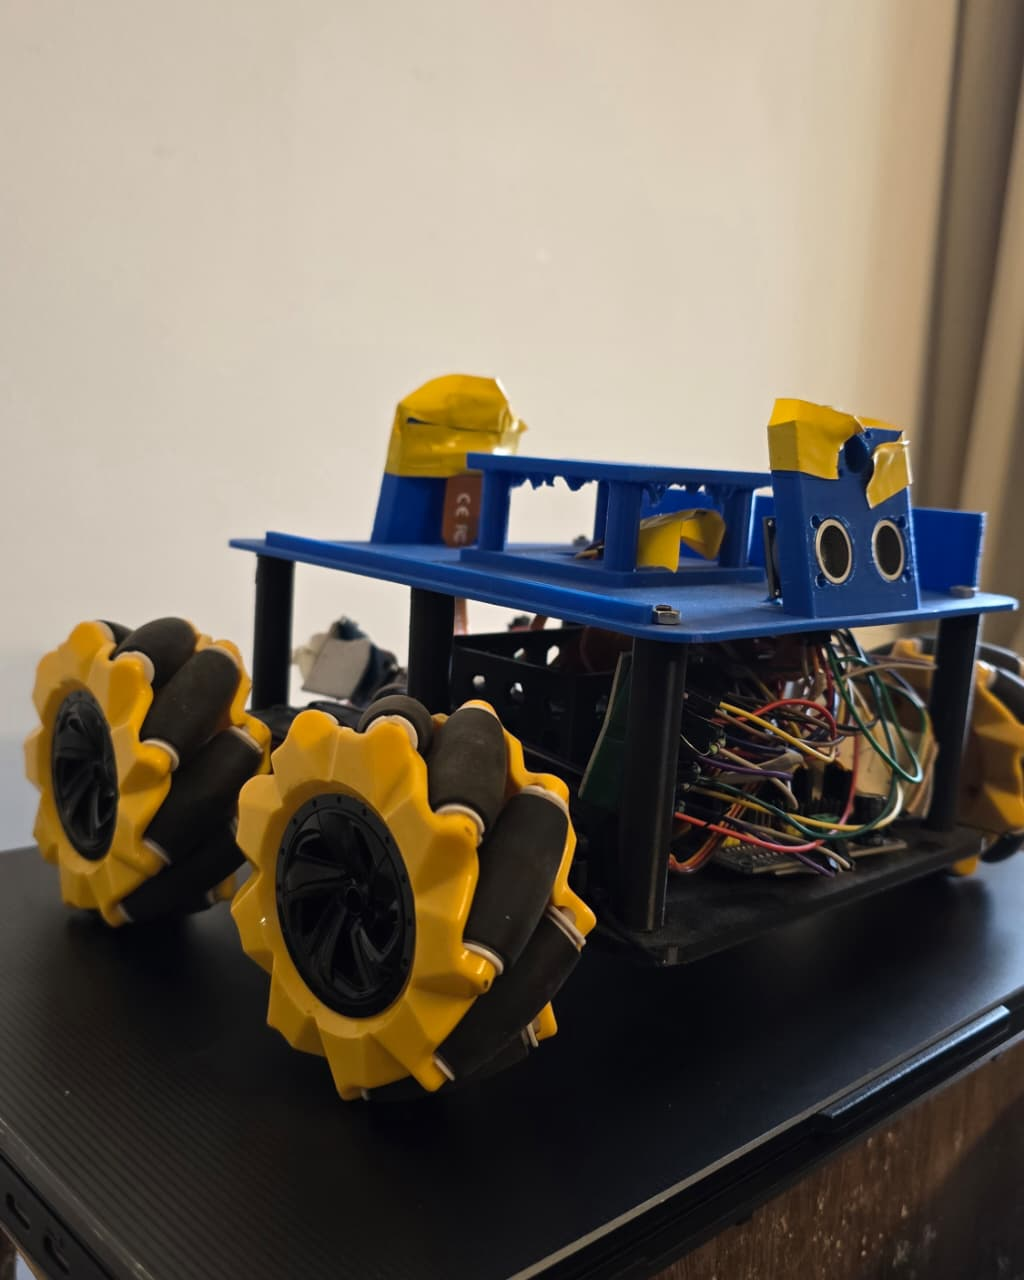
\includegraphics[width=0.62\textwidth]{Figures/Bot_view.jpeg}
    \caption{Assembled omnidirectional AMR prototype featuring the dual-deck chassis, four-wheel Mecanum drive train, front ultrasonic sensor bracket, upper sensing deck, and integrated electronics bay.}
    \label{fig:bot_view}
\end{figure}

\subsection{Hardware and Compute Interfacing}
The robot's computation and sensing stack comprises the following primary components:
\begin{enumerate}
    \item \textbf{Onboard Compute:} Raspberry Pi~5 (housed in the lower bay) executing a dedicated Python virtual environment (\texttt{robot\_env}) hosting low-level actuation scripts, sensory acquisition nodes, and SLAM pipelines.
    \item \textbf{Inertial Sensing:} An MPU-6050 6-axis sensor mounted on the upper deck and interfaced via I2C, acquiring 3-axis linear acceleration and 3-axis angular velocity data alongside onboard die temperature.
    \item \textbf{Ultrasonic Ranging:} A front-facing sonar module on the upper deck providing direct time-of-flight distance measurements for obstacle proximity alerts and reactive collision avoidance.
    \item \textbf{Dual-Camera Vision System:} A synchronized dual-camera setup positioned on the upper elevated bridge consisting of a primary forward-facing camera (\texttt{Cam~0}) and a secondary/stereo camera (\texttt{Cam~1}) for feature-based Visual SLAM and perception.
    \item \textbf{Power Monitoring:} An onboard voltage sensing divider continuously sampling battery supply voltage ($V_{\text{bat}}$) to track discharge characteristics during operation.
\end{enumerate}

\section{Omnidirectional Kinematic Modeling}
Unlike conventional differential drive architectures that are non-holonomic, the four-wheel Mecanum drive platform provides holonomic mobility. The robot can achieve independent linear translation along the longitudinal axis ($v_x$), lateral translation ($v_y$), and yaw rotational velocity ($\omega_z$) simultaneously without changing heading.

\subsection{Forward and Inverse Kinematics}
Let $r$ denote the radius of the Mecanum wheels, $l_x$ represent the longitudinal distance from the robot's center of mass to the wheel axes, and $l_y$ denote the lateral distance from the center of mass to the wheel centers. The inverse kinematic model maps desired body velocities $\mathbf{V} = [v_x, v_y, \omega_z]^T$ to the individual angular velocities of the four wheels $(\omega_1, \omega_2, \omega_3, \omega_4)$~\citep{siegwart2011introduction}:

\begin{equation}
\begin{bmatrix}
\omega_1 \\
\omega_2 \\
\omega_3 \\
\omega_4
\end{bmatrix}
= \frac{1}{r}
\begin{bmatrix}
1 & -1 & -(l_x + l_y) \\
1 &  1 &  (l_x + l_y) \\
1 &  1 & -(l_x + l_y) \\
1 & -1 &  (l_x + l_y)
\end{bmatrix}
\begin{bmatrix}
v_x \\
v_y \\
\omega_z
\end{bmatrix}
\label{eq:mecanum_kinematics}
\end{equation}

where $\omega_1$, $\omega_2$, $\omega_3$, and $\omega_4$ denote the angular velocities of the Front-Left, Front-Right, Rear-Left, and Rear-Right wheels, respectively.

By modulating individual motor directions and PWM duty cycles based on Eq.~(\ref{eq:mecanum_kinematics}), the platform executes six primary motion primitives: forward/backward translation, lateral strafing left/right, and in-place axial rotation.

\section{Low-Level Control, Calibration, and Teleoperation}
Low-level motion control and sensor interfacing are handled via dedicated Python modules within the onboard repository (\texttt{w\_move.py}, \texttt{move.py}, and \texttt{mpu6050.py}).

\subsection{Inertial Sensor Calibration and Teleoperation}
To mitigate sensor bias and temperature drift, an integrated MPU-6050 telemetry and teleoperation routine was developed. The script samples the accelerometer ($\text{m/s}^2$) and gyroscope ($\text{deg/s}$) across all three spatial axes while exposing a low-latency keyboard teleoperation matrix for manual system checkout.

\begin{figure}[htbp]
    \centering
    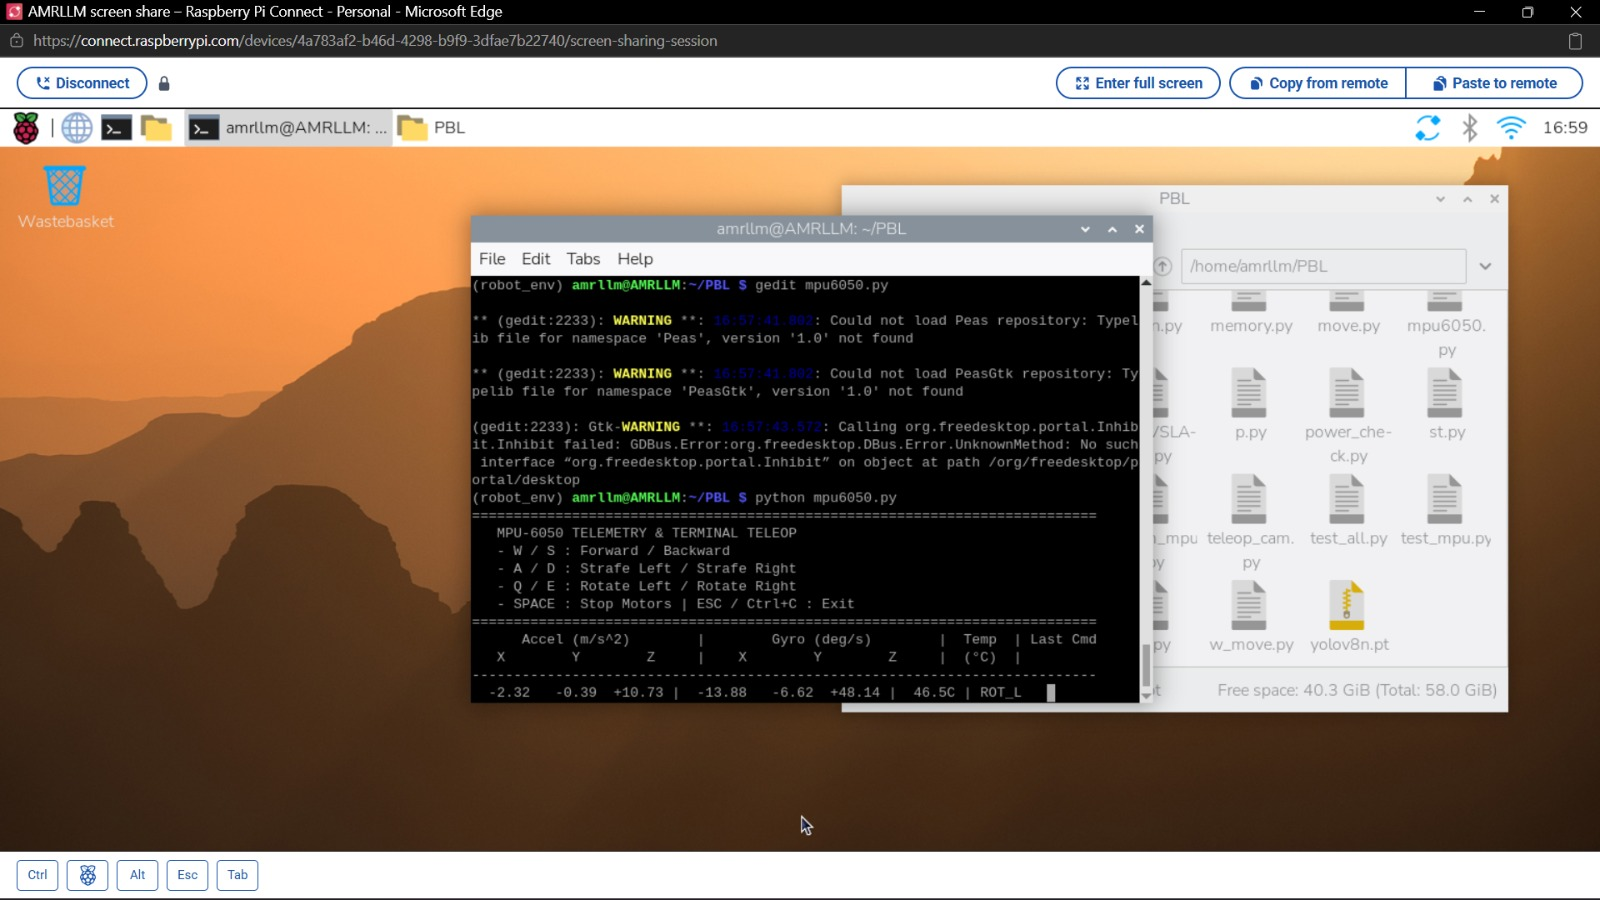
\includegraphics[width=0.85\textwidth]{Figures/GYRO_Callibration.jpeg}
    \caption{Real-time MPU-6050 IMU telemetry and terminal teleoperation interface running on the Raspberry Pi~5, displaying 3-axis acceleration, angular velocities, sensor temperature, and active motion command states.}
    \label{fig:gyro_calibration}
\end{figure}

As illustrated in Fig.~\ref{fig:gyro_calibration}, the teleoperation routine maps standardized control inputs:
\begin{itemize}
    \item \textbf{W / S:} Forward and backward longitudinal translation.
    \item \textbf{A / D:} Lateral strafe left and strafe right commands.
    \item \textbf{Q / E:} Counter-clockwise and clockwise rotational yaw commands.
    \item \textbf{Spacebar / Esc:} Instantaneous motor halt and routine termination.
\end{itemize}
The routine prints live inertial vectors, die temperature ($46.5^\circ\text{C}$), and the active actuation state (e.g., \texttt{ROT\_L}), ensuring motor command integrity and sensor health prior to autonomous routines.

\section{Visual SLAM and State Estimation}
Autonomous navigation without physical track constraints requires concurrent environmental mapping and ego-motion estimation~\citep{thrun2005probabilistic}. The platform deploys feature-based Visual SLAM (V-SLAM) leveraging the ORB-SLAM2 framework.

\subsection{ORB Feature Tracking and Map Point Generation}
The vision pipeline ingests real-time video frames from the primary camera (\texttt{Cam~0}) and stereo secondary camera (\texttt{Cam~1}) mounted on the upper deck. ORB (Oriented FAST and Rotated BRIEF) feature points are extracted across successive image frames. By computing FAST corners with orientation descriptors and matching corresponding BRIEF descriptors across baseline frames, the system computes:
\begin{enumerate}
    \item \textbf{Feature Landmark Triangulation:} Three-dimensional spatial coordinates for persistent visual landmarks across the environment.
    \item \textbf{Ego-Motion Estimation:} Motion transformations $[R | t]$ between consecutive frames, determining robot translation and yaw angle.
    \item \textbf{Bundle Adjustment:} Continuous optimization minimizing reprojection errors between observed feature locations and predicted landmark projections.
\end{enumerate}

\subsection{Real-Time Environmental Tracking and Telemetry Integration}
The V-SLAM pipeline executes concurrently on the Raspberry Pi~5, continuously estimating spatial poses ($X, Y, \text{Yaw}$), updating 3D landmark clouds, and acquiring forward ultrasonic range distances alongside battery state of charge. The full visualizer interface and experimental trajectory outcomes are presented and evaluated in Chapter~\ref{ch:results_and_discussion}.

\section{Vision-Based Object Detection}
In addition to geometric feature tracking, semantic environmental understanding is provided through an integrated YOLOv8 object detection model (\texttt{yolov8n.pt}) deployed within the onboard environment. By passing frames from the primary camera through the compact YOLOv8 network, the system detects and classifies key operational objects and obstacles in real time, supplying semantic labels to the spatial navigation memory.

\section{Natural Language Command Parsing Pipeline}
To bridge human operational commands with the autonomous navigation stack, the AMR incorporates an NLP/LLM interpretation engine~\citep{brown2020language, openai2024gpt}.

\subsection{Prompt Formatting and Entity Extraction}
Unstructured plain-English instructions entered by human operators (e.g., \textit{``Move forward to the inspection station''} or \textit{``Navigate to desk one''}) are processed via a structured prompt completion pipeline. The language model extracts two core parameters:
\begin{itemize}
    \item \textbf{Intent Classification:} Categorizing whether the command denotes a navigation task, a stop request, or a status query.
    \item \textbf{Target Entity Identification:} Isolating the specific semantic destination or landmark reference from conversational phrasing.
\end{itemize}

\subsection{Spatial Grounding via Topological Memory}
The parsed destination entity is cross-referenced against the local coordinate repository (\texttt{memory.py}). This database associates recognized semantic labels with calibrated Cartesian target poses $(x^*, y^*, \theta^*)$ previously registered within the SLAM map coordinate frame. Once matched, the target coordinates are passed directly to the onboard motion controller, which computes the required Mecanum velocity vectors to drive the robot to the goal pose while monitoring sonar thresholds for path clearance.

\section{Real-Time Operational Monitoring}
System health, pose tracking, and diagnostic telemetry are aggregated locally on the Raspberry Pi~5. The operational visualizer presents live metrics—including planar trajectories, active landmark clouds, battery discharge voltage, sonar range measurements, and motion states—directly within the desktop environment. This unified interface provides operators with complete supervisory visibility into both algorithmic SLAM execution and low-level electromechanical performance without loading the real-time control loop.
%! TEX root = ../main.tex
\chapter{Results and Discussion}
\label{ch:results_and_discussion}

This chapter presents the experimental evaluation and performance validation of the developed Autonomous Mobile Robot (AMR). The platform was evaluated across four functional dimensions: sensor calibration and teleoperation responsiveness, multi-camera Visual SLAM tracking and trajectory generation, real-time multi-modal telemetry integration, and semantic command interpretation with object detection.

\section{Inertial Sensor Calibration and Teleoperation Response}
Low-level actuation and sensor acquisition were validated using the interactive teleoperation and telemetry script (\texttt{mpu6050.py}) running within the onboard Python virtual environment on the Raspberry Pi~5.

\subsection{IMU Telemetry and Heading Response}
The MPU-6050 IMU, mounted on the upper deck, was continuously sampled across its 3-axis accelerometer and 3-axis gyroscope channels. During baseline static calibration, the vertical acceleration axis confirmed local gravity alignment ($a_z \approx +10.73\,\text{m/s}^2$) with minimal zero-bias error along the planar axes ($a_x = -2.32\,\text{m/s}^2, a_y = -0.39\,\text{m/s}^2$). 

During dynamic keyboard teleoperation testing, motion commands were dispatched to the motor driver to evaluate the Mecanum drive kinematic response:
\begin{itemize}
    \item \textbf{Longitudinal Locomotion (\texttt{W/S}):} Symmetrical forward and reverse translation verified balanced drive power delivery across all four wheels.
    \item \textbf{Lateral Strafing (\texttt{A/D}):} Reversing diagonal wheel pairs enabled zero-heading lateral displacement, confirming the 3-DOF holonomic capability of the platform.
    \item \textbf{Axial Rotation (\texttt{Q/E}):} During active counter-clockwise rotation (\texttt{ROT\_L}), the gyroscope registered an instantaneous rotational velocity of $\omega_z = +48.14^\circ/\text{s}$ (with planar angular rates of $\omega_x = -13.88^\circ/\text{s}$ and $\omega_y = -6.62^\circ/\text{s}$ reflecting dynamic chassis tilt).
    \item \textbf{Thermal Stability:} The onboard die temperature sensor maintained a stable operating range ($46.5^\circ\text{C}$) during extended motor switching cycles without requiring external active cooling.
\end{itemize}

\section{Visual SLAM Trajectory and Landmark Mapping}
Environmental mapping and state estimation were evaluated using the onboard feature-based Visual SLAM system. The robot executed exploratory runs in an indoor environment, combining the primary camera (\texttt{Cam~0}), stereo camera (\texttt{Cam~1}), and front sonar distance sensor.

\subsection{Trajectory Tracking and Landmark Point Distribution}
As the robot traversed the indoor testing space, ORB feature extraction generated a continuous map of triangulated 3D landmark points.

\begin{figure}[htbp]
    \centering
    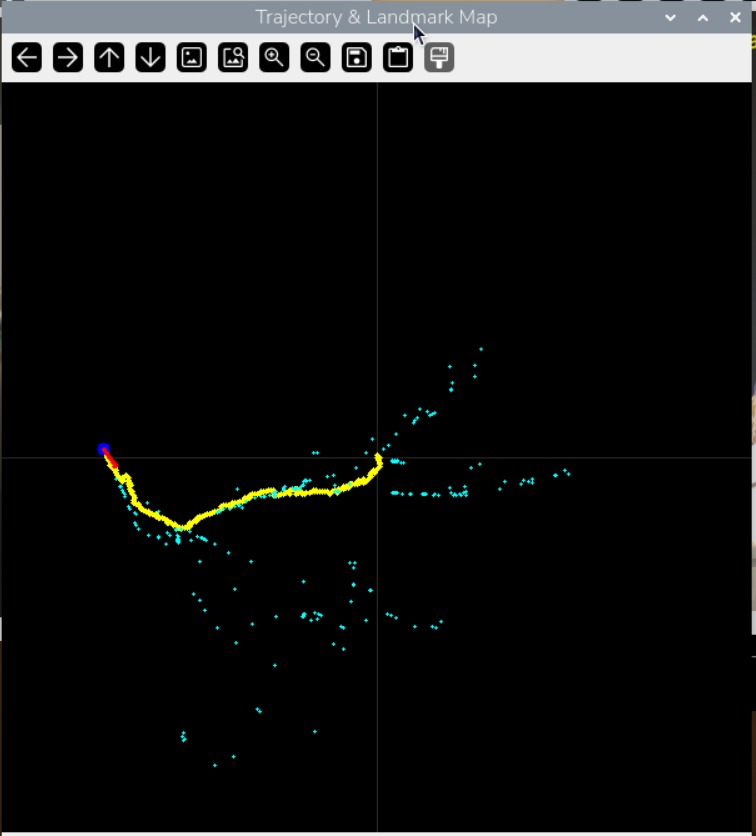
\includegraphics[width=0.78\textwidth]{Figures/Basic_MAP.jpeg}
    \caption{Trajectory plot and sparse landmark feature distribution generated during the indoor visual navigation run.}
    \label{fig:basic_map}
\end{figure}

Fig.~\ref{fig:basic_map} illustrates the reconstructed path trajectory and associated landmark feature cloud:
\begin{itemize}
    \item The yellow path denotes the continuous trajectory estimated from consecutive visual frame transformations.
    \item The cyan points represent persistent environmental landmarks extracted and triangulated from scene geometry.
    \item The blue marker indicates the active robot pose, while red vector segments illustrate instantaneous velocity vectors during heading adjustments.
\end{itemize}

\subsection{Multi-Camera Tracking Performance}
Fig.~\ref{fig:map_two_cameras} demonstrates the real-time V-SLAM tracking session running under Raspberry Pi Connect.

\begin{figure}[htbp]
    \centering
    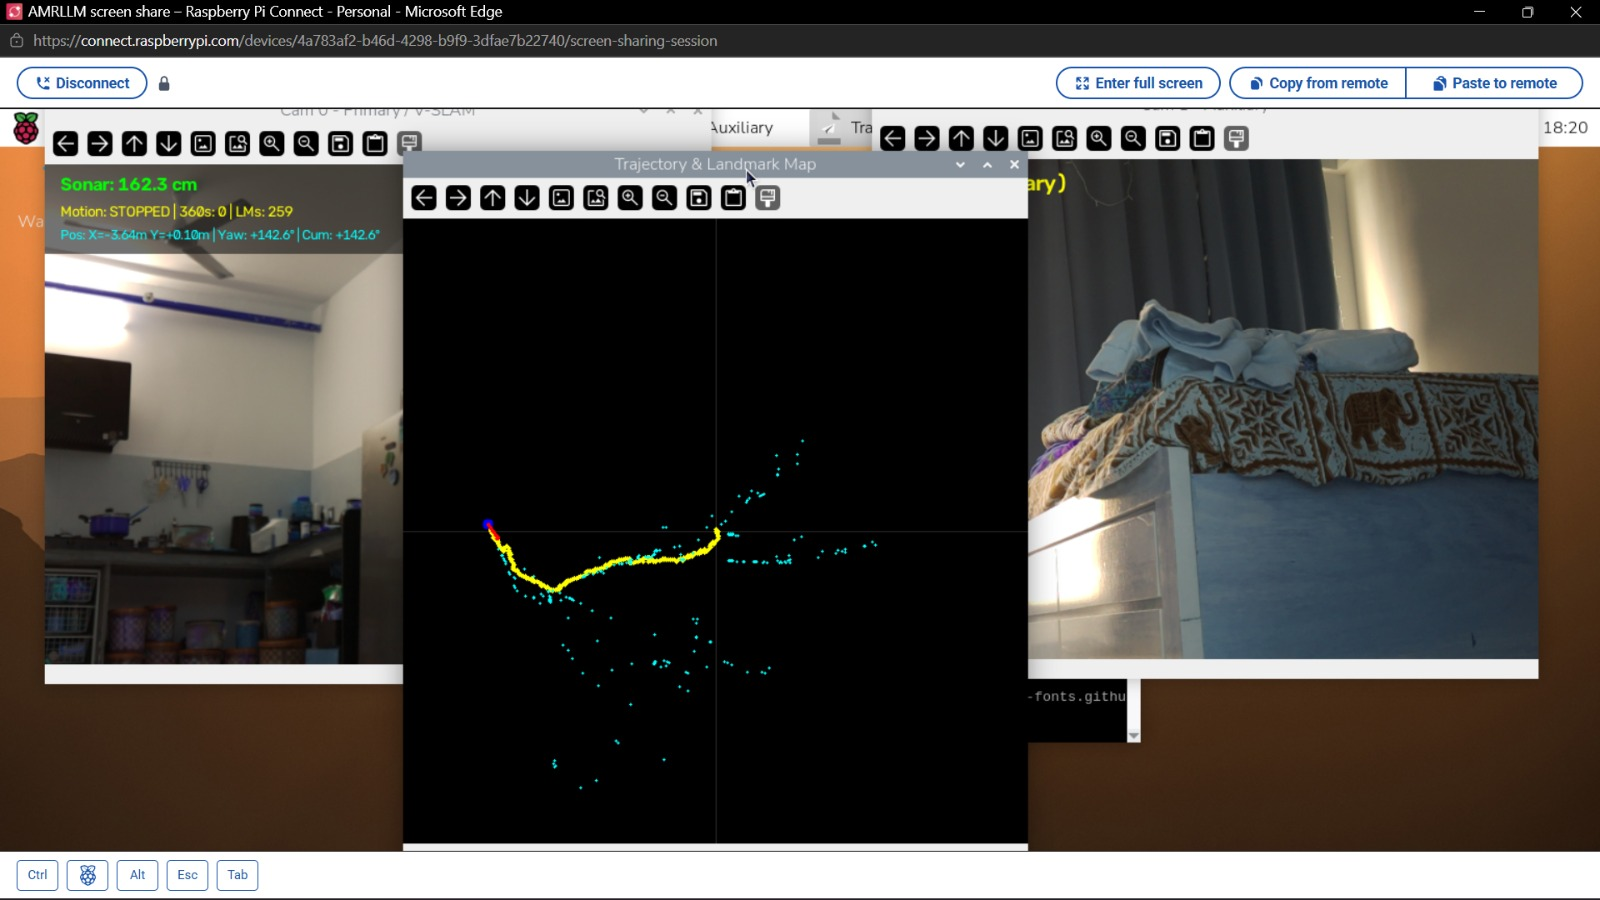
\includegraphics[width=0.88\textwidth]{Figures/Map_with_two_cam.jpeg}
    \caption{Real-time V-SLAM tracking session displaying dual camera feedback, ultrasonic distance ranging ($162.3\,\text{cm}$), tracked visual landmarks ($259$ points), and pose coordinates.}
    \label{fig:map_two_cameras}
\end{figure}

During this initial exploration run:
\begin{itemize}
    \item The system tracked $259$ active visual landmarks (\texttt{LMs: 259}) across the field of view.
    \item The estimated spatial coordinates converged to $X = -3.64\,\text{m}$ and $Y = +0.10\,\text{m}$, with a cumulative orientation of $\text{Yaw} = +142.6^\circ$.
    \item The front ultrasonic sensor maintained concurrent distance measurements, registering an obstacle clearance of $162.3\,\text{cm}$.
\end{itemize}

\section{Integrated System Performance and Telemetry Overlay}
Extended autonomous navigation trials evaluated tracking stability, feature retention, and multi-sensor telemetry integration.

\begin{figure}[htbp]
    \centering
    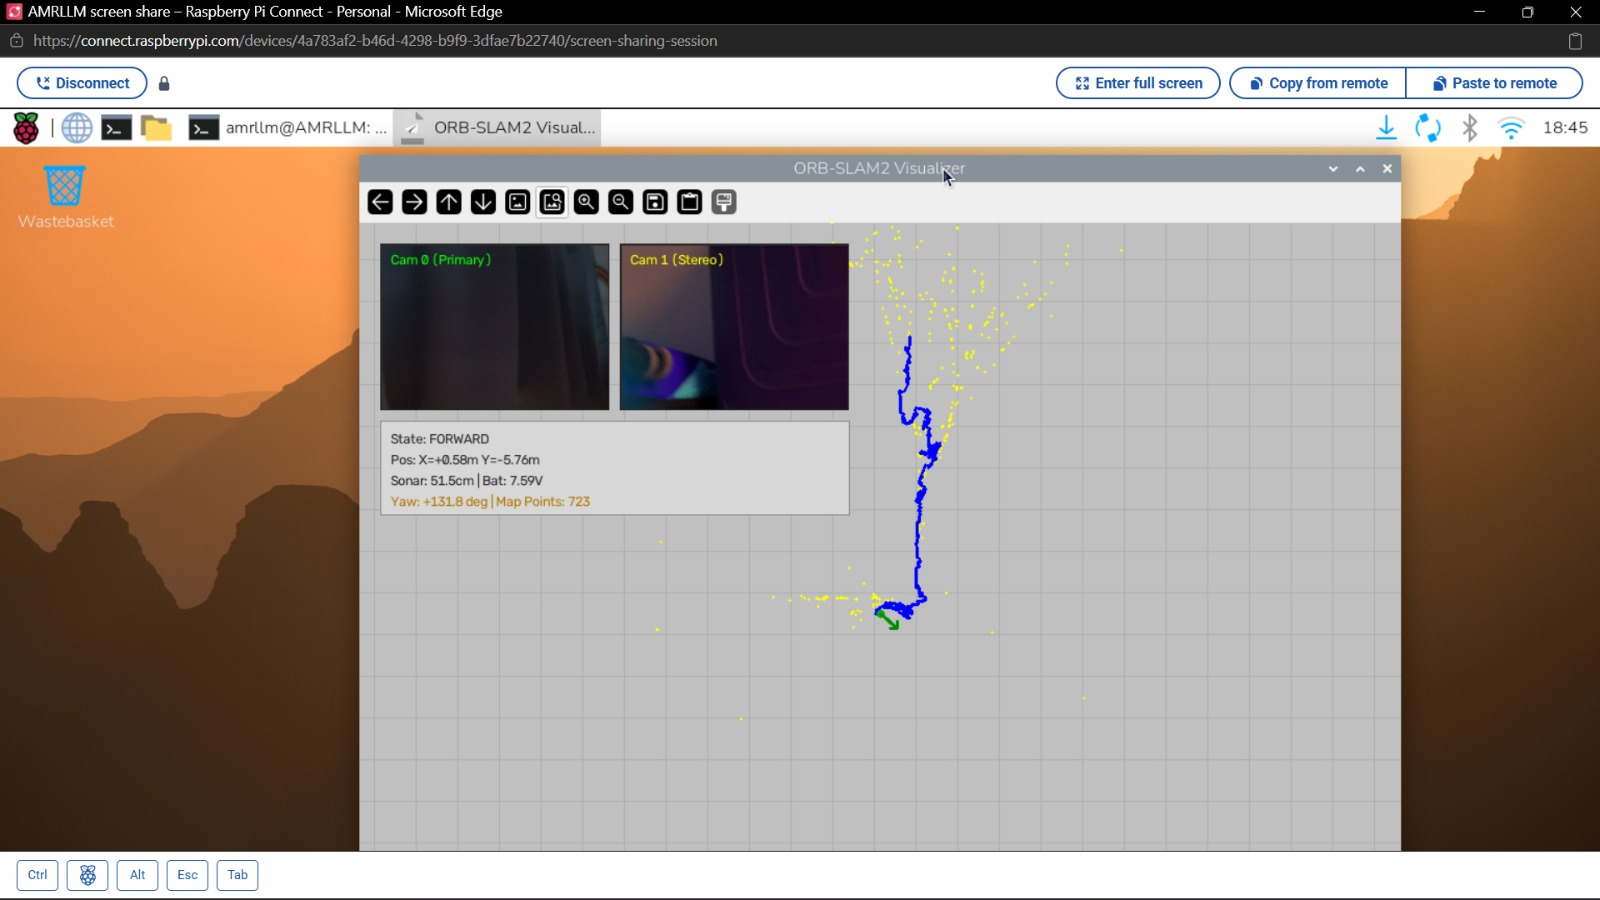
\includegraphics[width=0.92\textwidth]{Figures/SLAM_with_ORB.jpeg}
    \caption{ORB-SLAM2 visualizer session showing dual-camera visual feature processing, tracking across $723$ map points, and real-time operational telemetry overlay.}
    \label{fig:slam_orb}
\end{figure}

As shown in Fig.~\ref{fig:slam_orb}, the ORB-SLAM2 visualizer maintained tracking continuity during extended path traversal:
\begin{itemize}
    \item \textbf{Map Scale and Point Density:} Active tracked map points increased to $723$ points, providing a dense geometric representation of the surrounding walls, furniture, and obstacles.
    \item \textbf{Ego-Motion Estimation:} The platform tracked an extended trajectory reaching Cartesian coordinates of $X = +0.58\,\text{m}, Y = -5.76\,\text{m}$ with a heading angle of $+131.8^\circ$ while executing a sustained \texttt{FORWARD} translation.
    \item \textbf{Proximity Obstacle Detection:} As the platform approached forward boundaries, the ultrasonic sonar registered obstacle proximity down to $51.5\,\text{cm}$, demonstrating reliable obstacle detection within the forward blind spot of the cameras.
    \item \textbf{Power Rail Telemetry:} Real-time voltage sensing reported a battery potential of $7.59\,\text{V}$, confirming adequate operational headroom above the low-voltage cutoff threshold during simultaneous motor driving and compute workloads.
\end{itemize}

\section{Object Detection and Semantic Grounding Validation}
The vision and language pipeline was evaluated by pairing YOLOv8 real-time object classification with topological waypoint dispatch.

\subsection{Object Detection via YOLOv8}
The lightweight \texttt{yolov8n.pt} model executed directly on the primary camera feed on the Raspberry Pi~5. The network successfully identified operational targets and obstacles—such as chairs, desks, and persons—within the camera frame, providing contextual validation of landmark locations mapped in the spatial visualizer.

\subsection{Natural Language Command Parsing}
Natural language instructions entered through the console or dispatched to the local HTTP endpoint (\texttt{http://127.0.0.1:8000/send-command}) were evaluated across varying phrasings. Table~\ref{tab:nlp_performance} summarizes representative test cases evaluated by the language interpretation pipeline.

\begin{table}[htbp]
\centering
\small
\caption{Natural language command parsing and destination extraction results.}
\label{tab:nlp_performance}
\renewcommand{\arraystretch}{1.3}
\begin{tabularx}{\textwidth}{>{\raggedright\arraybackslash}X >{\raggedright\arraybackslash}p{2.6cm} >{\raggedright\arraybackslash}p{2.8cm} >{\raggedright\arraybackslash}p{2.6cm}}
\hline
\textbf{Operator Command Input} & \textbf{Identified Intent} & \textbf{Extracted Entity} & \textbf{Target Pose ($X, Y$)} \\ \hline
``Navigate to the charging station'' & \texttt{NAVIGATE} & \texttt{charging\_station} & $(+0.50\,\text{m}, -5.50\,\text{m})$ \\ \hline
``Go to desk one'' & \texttt{NAVIGATE} & \texttt{desk\_1} & $(-3.50\,\text{m}, +0.20\,\text{m})$ \\ \hline
``Move forward and halt'' & \texttt{MOVE\_STEP} & \texttt{forward} & Relative Step \\ \hline
``Stop all motors immediately'' & \texttt{EMERGENCY\_STOP} & \texttt{none} & Actuator Halt \\ \hline
``I need you to navigate to somewhere else'' & \texttt{NAVIGATE} & \texttt{none} & Rejection / Safe Halt \\ \hline
\end{tabularx}
\end{table}

The entity extraction pipeline reliably isolated target labels from unambiguous conversational text. Extracted labels were cross-referenced with pre-registered coordinate tuples stored in \texttt{memory.py}, enabling the platform to set deterministic destination coordinates corresponding to its internal visual map frame.

To evaluate system safety against ambiguous or out-of-vocabulary instructions, arbitrary commands were sent directly to the local REST endpoint:

\begin{verbatim}
$ curl -X POST "http://127.0.0.1:8000/send-command" \
       -H "Content-Type: application/json" \
       -d '{"text": "I need you to navigate to somewhere else"}'

{"target":"none"}
\end{verbatim}

As demonstrated above, when the pipeline receives an ungrounded directive without a valid registered destination, it safely returns \texttt{\{"target":"none"\}}. This ensures that spurious or ambiguous commands do not trigger unverified coordinate trajectories.

\section{Summary of Experimental Observations}
Table~\ref{tab:experimental_summary} consolidates the operational metrics recorded across the testing sessions.

\begin{table}[htbp]
\centering
\small
\caption{Summary of experimental operating metrics recorded during system evaluation.}
\label{tab:experimental_summary}
\renewcommand{\arraystretch}{1.3}
\begin{tabularx}{\textwidth}{>{\raggedright\arraybackslash}p{4.2cm} >{\raggedright\arraybackslash}X >{\raggedright\arraybackslash}p{4.0cm}}
\hline
\textbf{Subsystem Parameter} & \textbf{Observed Metric / Value} & \textbf{Operational Status} \\ \hline
Locomotion Modes & Forward, Strafe (L/R), Rotate (L/R) & Verified via Mecanum kinematics \\ \hline
Gyroscope Angular Velocity & Up to $+48.14^\circ/\text{s}$ ($\omega_z$) & Real-time I2C telemetry \\ \hline
Sensor Die Temperature & $46.5^\circ\text{C}$ & Thermally stable under load \\ \hline
Visual Map Point Density & $259$ to $723$ landmarks & Stable tracking without divergence \\ \hline
Estimated Pose Envelope & $X \in [-3.64, +0.58]\,\text{m}$, $Y \in [-5.76, +0.10]\,\text{m}$ & Bounded indoor test arena \\ \hline
Ultrasonic Ranging Envelope & $51.5\,\text{cm}$ to $162.3\,\text{cm}$ & Active forward obstacle detection \\ \hline
Operational Supply Voltage & $7.59\,\text{V}$ & Adequate logic and drive power \\ \hline
Object Detection Network & YOLOv8 Nano (\texttt{yolov8n.pt}) & Real-time semantic tagging \\ \hline
\end{tabularx}
\end{table} %D1
%! TEX root = ../main.tex
\chapter{Work to be Done}
\label{ch:work_to_be_done}
\label{Ch_6_Work to be done}

\section{Introduction}
This chapter outlines the remaining development, integration, and validation tasks for the completion of the Autonomous Mobile Robot (AMR) project. The proposed schedule is divided into four targeted phases: foundational platform and navigation setup (Phase~1), operational telemetry and cloud dashboard integration (Phase~2), natural language goal translation and closed-loop dispatch (Phase~3), and comprehensive system validation (Testing).

\section{Planned Work}
The remaining engineering work is structured into eleven specific work packages across four distinct project phases:

\subsection*{Phase 1: Autonomous Navigation and Platform Setup}
\begin{itemize}
    \item \textbf{T1.1 --- Chassis Assembly \& Motor Driver Setup:} Complete structural fabrication and mechanical assembly. The structural platform utilizes a 6\,mm ABS lower base plate printed at 15\% infill for chassis rigidity, a 4\,mm PLA upper deck printed at 10\% infill to minimize upper-deck inertia, and solid 100\% infill ABS motor-to-wheel shaft couplers to withstand high torsional loads from the Mecanum wheels. Wire all drive motors to the motor drivers and configure low-level directional actuation and PWM velocity control.
    \item \textbf{T1.2 --- Sensor Integration (LiDAR/Camera \& Microcontroller):} Interface the perception and inertial sensors (LiDAR/cameras, MPU-6050 IMU, and ultrasonic rangefinder) with the onboard compute and microcontroller platforms.
    \item \textbf{T1.3 --- SLAM Environment Mapping \& Costmaps:} Execute exploratory indoor runs to generate high-resolution occupancy grid maps, configure inflation layers, and establish dynamic local/global costmaps.
    \item \textbf{T1.4 --- Path Planner Tuning \& Avoidance:} Tune global path planning ($A^*$/NavFn) and local trajectory optimization controllers for reliable dynamic obstacle avoidance.
\end{itemize}

\subsection*{Phase 2: Telemetry and Dashboard Infrastructure}
\begin{itemize}
    \item \textbf{T2.1 --- Sensor Telemetry Extraction (Voltage/Speed):} Implement onboard background daemons to sample battery supply voltage, wheel encoder velocities, and system health metrics at high frequency.
    \item \textbf{T2.2 --- MQTT / Wireless Communication Bridge:} Establish an event-driven pub/sub messaging bridge over Wi-Fi to serialize and stream telemetry packets asynchronously without blocking real-time motion control.
    \item \textbf{T2.3 --- DAS Database Server Setup:} Deploy a Data Acquisition Server (DAS) database backend to ingest, log, and structure continuous runtime telemetry streams.
    \item \textbf{T2.4 --- Power BI Operational Dashboard Build:} Construct an interactive, browser-accessible Power BI dashboard providing remote supervisors with real-time visual tracking of robot speed, battery curves, and active coordinate status.
\end{itemize}

\subsection*{Phase 3: Natural Language Processing and Semantic Dispatch}
\begin{itemize}
    \item \textbf{T3.1 --- LLM API / Light NLP Pipeline Integration:} Configure a lightweight NLP and Large Language Model prompt completion pipeline to parse unstructured operator voice/text commands into structured intent and entity tags.
    \item \textbf{T3.2 --- Spatial Map Database \& Coordinate Mapping:} Construct a local topological database associating common landmark and room names with calibrated Cartesian poses $(x, y, \theta)$ on the navigation map.
    \item \textbf{T3.3 --- Goal Dispatch \& End-to-End Control Loop:} Close the high-level loop by automatically passing parsed coordinate goals into the navigation action client to initiate autonomous locomotion.
\end{itemize}

\subsection*{Testing: Verification and Academic Synthesis}
\begin{itemize}
    \item \textbf{T4.1 --- System Validation \& Report:} Perform exhaustive multi-run navigation trials, assess command translation accuracy and telemetry latency, and synthesize final documentation for the project report.
\end{itemize}

\section{Timeline}
The project timeline is organized into 5-day intervals spanning from August 1 to October 15. Table~\ref{tab:project_schedule} summarizes the task duration windows, and Fig.~\ref{fig:project_gantt} illustrates the operational Gantt chart.

\begin{table}[htbp]
\centering
\small
\caption{Detailed task breakdown and execution windows across project phases.}
\label{tab:project_schedule}
\renewcommand{\arraystretch}{1.25}
\begin{tabularx}{\textwidth}{>{\raggedright\arraybackslash}p{1.8cm} >{\raggedright\arraybackslash}p{1.4cm} >{\raggedright\arraybackslash}X >{\raggedright\arraybackslash}p{3.2cm}}
\hline
\textbf{Phase} & \textbf{Task ID} & \textbf{Task Description} & \textbf{Timeline Window} \\ \hline
\multirow{4}{*}{\textbf{Phase 1}} 
 & T1.1 & Chassis Assembly \& Motor Driver Setup & Aug 1 -- Aug 10 \\ \cline{2-4}
 & T1.2 & Sensor Integration (LiDAR/Cam \& MCU) & Aug 6 -- Aug 20 \\ \cline{2-4}
 & T1.3 & SLAM Environment Mapping \& Costmaps & Aug 16 -- Aug 30 \\ \cline{2-4}
 & T1.4 & Path Planner Tuning \& Avoidance & Aug 26 -- Sep 10 \\ \hline
\multirow{4}{*}{\textbf{Phase 2}} 
 & T2.1 & Sensor Telemetry Extraction (Voltage/Speed) & Sep 1 -- Sep 10 \\ \cline{2-4}
 & T2.2 & MQTT / Wireless Communication Bridge & Sep 6 -- Sep 20 \\ \cline{2-4}
 & T2.3 & DAS Database Server Setup & Sep 11 -- Sep 20 \\ \cline{2-4}
 & T2.4 & Power BI Operational Dashboard Build & Sep 16 -- Sep 30 \\ \hline
\multirow{3}{*}{\textbf{Phase 3}} 
 & T3.1 & LLM API / Light NLP Integration & Sep 21 -- Oct 5 \\ \cline{2-4}
 & T3.2 & Spatial Map DB \& Coordinates & Sep 26 -- Oct 10 \\ \cline{2-4}
 & T3.3 & Goal Dispatch \& Control Loop & Oct 6 -- Oct 15 \\ \hline
\textbf{Testing} 
 & T4.1 & System Validation \& Report & Oct 11 -- Oct 15 \\ \hline
\end{tabularx}
\end{table}

\begin{figure}[htbp]
\centering
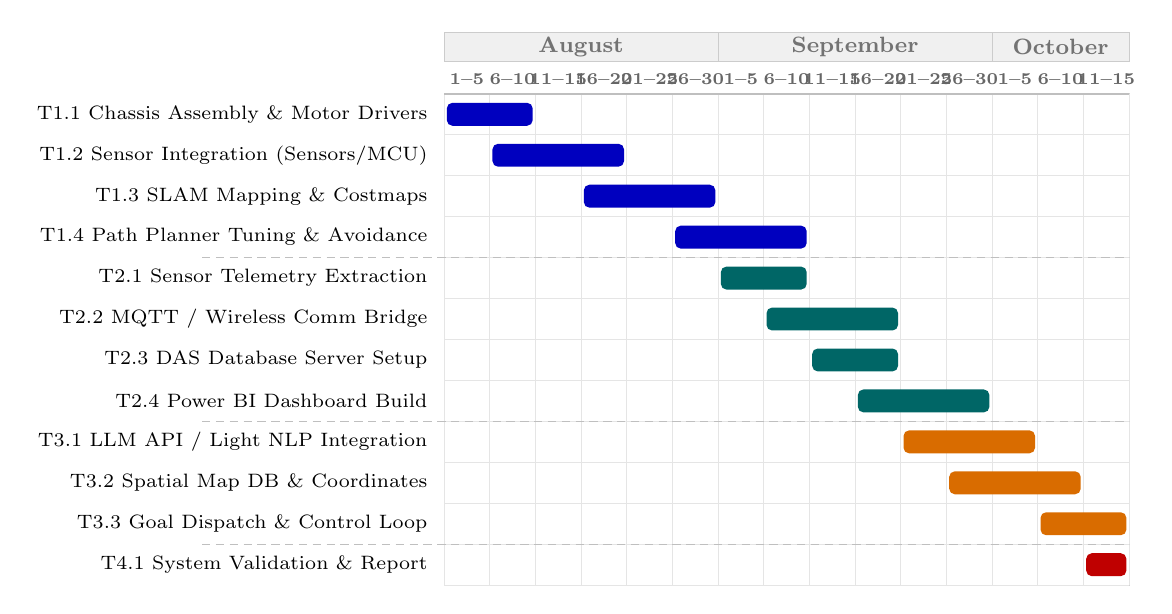
\begin{tikzpicture}[x=0.58cm, y=0.52cm]
    \draw[draw=gray!35, fill=white] (0,0) rectangle (15,12);
    \draw[help lines, color=gray!20, line width=0.35pt] (0,0) grid[xstep=1, ystep=1] (15,12);

    % Month Header Banners
    \draw[fill=gray!12, draw=gray!40, line width=0.4pt] (0, 12.8) rectangle (6, 13.5);
    \node[font=\footnotesize\bfseries, text=gray!90!black] at (3, 13.15) {August};

    \draw[fill=gray!12, draw=gray!40, line width=0.4pt] (6, 12.8) rectangle (12, 13.5);
    \node[font=\footnotesize\bfseries, text=gray!90!black] at (9, 13.15) {September};

    \draw[fill=gray!12, draw=gray!40, line width=0.4pt] (12, 12.8) rectangle (15, 13.5);
    \node[font=\footnotesize\bfseries, text=gray!90!black] at (13.5, 13.15) {October};

    % 5-Day Interval Headers
    \foreach \i/\label in {
        0.5/{1--5}, 1.5/{6--10}, 2.5/{11--15}, 3.5/{16--20}, 4.5/{21--25}, 5.5/{26--30},
        6.5/{1--5}, 7.5/{6--10}, 8.5/{11--15}, 9.5/{16--20}, 10.5/{21--25}, 11.5/{26--30},
        12.5/{1--5}, 13.5/{6--10}, 14.5/{11--15}
    } {
        \node[font=\fontsize{6}{7}\selectfont\bfseries, text=gray!80!black] at (\i, 12.35) {\label};
    }
    \draw[line width=0.5pt, color=gray!50] (0, 12) -- (15, 12);

    % Task Labels
    \node[anchor=east, font=\scriptsize] at (-0.15, 11.5) {T1.1 Chassis Assembly \& Motor Drivers};
    \node[anchor=east, font=\scriptsize] at (-0.15, 10.5) {T1.2 Sensor Integration (Sensors/MCU)};
    \node[anchor=east, font=\scriptsize] at (-0.15, 9.5) {T1.3 SLAM Mapping \& Costmaps};
    \node[anchor=east, font=\scriptsize] at (-0.15, 8.5) {T1.4 Path Planner Tuning \& Avoidance};

    \node[anchor=east, font=\scriptsize] at (-0.15, 7.5) {T2.1 Sensor Telemetry Extraction};
    \node[anchor=east, font=\scriptsize] at (-0.15, 6.5) {T2.2 MQTT / Wireless Comm Bridge};
    \node[anchor=east, font=\scriptsize] at (-0.15, 5.5) {T2.3 DAS Database Server Setup};
    \node[anchor=east, font=\scriptsize] at (-0.15, 4.5) {T2.4 Power BI Dashboard Build};

    \node[anchor=east, font=\scriptsize] at (-0.15, 3.5) {T3.1 LLM API / Light NLP Integration};
    \node[anchor=east, font=\scriptsize] at (-0.15, 2.5) {T3.2 Spatial Map DB \& Coordinates};
    \node[anchor=east, font=\scriptsize] at (-0.15, 1.5) {T3.3 Goal Dispatch \& Control Loop};

    \node[anchor=east, font=\scriptsize] at (-0.15, 0.5) {T4.1 System Validation \& Report};

    % Phase Dividing Grid Lines
    \draw[densely dashed, color=gray!50, line width=0.4pt] (-5.3, 8) -- (15, 8);
    \draw[densely dashed, color=gray!50, line width=0.4pt] (-5.3, 4) -- (15, 4);
    \draw[densely dashed, color=gray!50, line width=0.4pt] (-5.3, 1) -- (15, 1);

    % Phase 1 Bars
    \fill[rounded corners=2pt, fill=blue!75!black] (0.06, 11.22) rectangle (1.94, 11.78);
    \fill[rounded corners=2pt, fill=blue!75!black] (1.06, 10.22) rectangle (3.94, 10.78);
    \fill[rounded corners=2pt, fill=blue!75!black] (3.06, 9.22) rectangle (5.94, 9.78);
    \fill[rounded corners=2pt, fill=blue!75!black] (5.06, 8.22) rectangle (7.94, 8.78);

    % Phase 2 Bars
    \fill[rounded corners=2pt, fill=teal!80!black] (6.06, 7.22) rectangle (7.94, 7.78);
    \fill[rounded corners=2pt, fill=teal!80!black] (7.06, 6.22) rectangle (9.94, 6.78);
    \fill[rounded corners=2pt, fill=teal!80!black] (8.06, 5.22) rectangle (9.94, 5.78);
    \fill[rounded corners=2pt, fill=teal!80!black] (9.06, 4.22) rectangle (11.94, 4.78);

    % Phase 3 Bars
    \fill[rounded corners=2pt, fill=orange!85!black] (10.06, 3.22) rectangle (12.94, 3.78);
    \fill[rounded corners=2pt, fill=orange!85!black] (11.06, 2.22) rectangle (13.94, 2.78);
    \fill[rounded corners=2pt, fill=orange!85!black] (13.06, 1.22) rectangle (14.94, 1.78);

    % Testing Bar
    \fill[rounded corners=2pt, fill=red!75!black] (14.06, 0.22) rectangle (14.94, 0.78);
\end{tikzpicture}
\caption{Gantt chart illustrating the schedule and task distribution from August 1 to October 15.}
\label{fig:project_gantt}
\end{figure}

\section{Expected Outcomes}
Execution of the planned timeline will yield the following verified outcomes:
\begin{enumerate}
    \item \textbf{Autonomous Navigation Platform:} An operational AMR platform navigating dynamically within mapped environments using calibrated SLAM and obstacle costmaps.
    \item \textbf{Unified Cloud Telemetry Monitoring:} Continuous streaming of battery health, velocity vectors, and operational coordinates to a Power BI supervisory dashboard via an MQTT/wireless bridge.
    \item \textbf{Natural Language Dispatch System:} An end-to-end command interpretation loop allowing non-specialist users to dispatch spatial navigation goals via conversational text.
    \item \textbf{Comprehensive Performance Evaluation:} Documented empirical benchmarks detailing path tracking repeatability, telemetry latency, and obstacle avoidance response.
\end{enumerate} %D2
%\include{Chapters/CH7_FE_FS} %D3
%\include{Chapters/CH8_TrAdaBoost} %
%\include{Chapters/CH9_RTNN} % Conclusion and future work
%\include{Chapters/Ch10_Conclusions}
%%%%%%%%%%%%%%%%%%%%%%%%%%%%%%%%%%%%%%%%%%%%%%%%%%%%%%%%%%%%%%%%%%%%%%%%
\newpage
\addcontentsline{toc}{chapter}{References}
%\bibliographystyle{apalike}

\bibliography{references}
\clearpage
\pagebreak
\let\svaddcontentsline\addcontentsline
\renewcommand\addcontentsline[3]{%
  \ifthenelse{\equal{#1}{lof}}{}%
  {\ifthenelse{\equal{#1}{lot}}{}{\svaddcontentsline{#1}{#2}{#3}}}}
%! TEX root = ../main.tex
\chapter*{Annexure I: Design Data}
\addcontentsline{toc}{chapter}{Annexure I: Design Data}

% Change numbering style for sections, figures, tables, equations
\renewcommand{\thesection}{I.\arabic{section}}
\renewcommand{\thefigure}{I.\arabic{figure}}
\renewcommand{\thetable}{I.\arabic{table}}
\renewcommand{\theequation}{I.\arabic{equation}}

% Reset counters so numbering starts fresh
\setcounter{section}{0}
\setcounter{figure}{0}
\setcounter{table}{0}
\setcounter{equation}{0}

\section{Introduction}
This annexure contains detailed design data used in the project, including structural material specifications, 3D printing parameters, kinematic equations, and electromechanical parameters for the Autonomous Mobile Robot (AMR).

\section*{Design Specifications}
\begin{table}[htbp]
    \centering
    \caption{Design Specifications for the AMR Platform}
    \label{tab:system_design_specs}
    \renewcommand{\arraystretch}{1.3}
    \begin{tabular}{|p{5.5cm}|p{8.5cm}|}
        \hline
        \textbf{Parameter} & \textbf{Value / Specification} \\ \hline
        Chassis Structure & Dual-tier modular chassis with vertical standoffs \\ \hline
        Drive Configuration & 4-wheel independent Mecanum drive (holonomic, 3-DOF) \\ \hline
        Lower Base Plate & 6\,mm ABS (15\% infill density) \\ \hline
        Upper Sensing Deck & 4\,mm PLA (10\% infill density) \\ \hline
        Motor Shaft Couplers & Solid ABS (100\% infill density) \\ \hline
        Primary Compute & Raspberry Pi 5 (housed in lower bay) \\ \hline
        Inertial Measurement Unit & MPU-6050 6-axis IMU (mounted on upper deck) \\ \hline
        Ranging Sensor & Front ultrasonic distance sensor (mounted on upper deck) \\ \hline
        Vision System & Dual cameras (Cam 0 Primary, Cam 1 Stereo on upper deck bridge) \\ \hline
        Operating Potential & 7.4\,V nominal Li-ion pack (7.59\,V verified baseline) \\ \hline
    \end{tabular}
\end{table}

\section{Design Calculations}
Key calculations performed for chassis locomotion, motor velocity matching, and normal load distribution:

\subsection*{Mecanum Drive Inverse Kinematics}
For a four-wheel Mecanum drive with wheel radius $r$, longitudinal half-length $l_x$, and lateral half-width $l_y$, the individual wheel rotational speeds $(\omega_1, \omega_2, \omega_3, \omega_4)$ required to generate body velocities $(v_x, v_y, \omega_z)$ are given by:

\begin{equation}
    \begin{bmatrix}
        \omega_1 \\
        \omega_2 \\
        \omega_3 \\
        \omega_4
    \end{bmatrix}
    = \frac{1}{r}
    \begin{bmatrix}
        1 & -1 & -(l_x + l_y) \\
        1 &  1 &  (l_x + l_y) \\
        1 &  1 & -(l_x + l_y) \\
        1 & -1 &  (l_x + l_y)
    \end{bmatrix}
    \begin{bmatrix}
        v_x \\
        v_y \\
        \omega_z
    \end{bmatrix}
\end{equation}

Where:
\begin{itemize}
    \item $\omega_1, \omega_2, \omega_3, \omega_4$ = angular velocities of front-left, front-right, rear-left, and rear-right wheels ($\text{rad/s}$)
    \item $v_x, v_y$ = longitudinal and lateral chassis velocities ($\text{m/s}$)
    \item $\omega_z$ = yaw rotational velocity ($\text{rad/s}$)
    \item $r$ = outer radius of the Mecanum wheels ($\text{m}$)
    \item $l_x, l_y$ = distance from the robot center of mass to the wheel contact centers along $X$ and $Y$ axes ($\text{m}$)
\end{itemize}

\subsection*{Chassis Linear Velocity from Motor Output}
The maximum theoretical longitudinal speed $v_{\text{max}}$ in pure forward locomotion ($v_y = 0, \omega_z = 0$) is determined from the motor gearbox rotational speed $N$:

\begin{equation}
    v_{\text{max}} = \left( \frac{2 \pi N}{60} \right) \cdot r
\end{equation}

Where:
\begin{itemize}
    \item $v_{\text{max}}$ = maximum linear chassis velocity ($\text{m/s}$)
    \item $N$ = motor output rotational speed ($\text{RPM}$)
    \item $r$ = Mecanum wheel radius ($\text{m}$)
\end{itemize}

\subsection*{Static Normal Load Distribution}
Assuming symmetric mass distribution across the chassis tiers, the static normal force $F_N$ borne by each wheel contact interface is:

\begin{equation}
    F_{N} = \frac{m \cdot g}{4}
\end{equation}

Where:
\begin{itemize}
    \item $F_N$ = static normal reaction force per wheel ($\text{N}$)
    \item $m$ = total robot mass ($\text{kg}$)
    \item $g$ = acceleration due to gravity ($9.81\,\text{m/s}^2$)
\end{itemize}

\section{Additional Data}
\begin{itemize}
    \item \textbf{Additive Manufacturing Tolerances:} $\pm 0.20\,\text{mm}$ clearance on motor shaft apertures, mounting holes, and standoff slots.
    \item \textbf{Thermal Slicing Parameters:}
    \begin{itemize}
        \item Lower Base Plate \& Couplers (ABS): Nozzle $240^\circ\text{C}$, Bed $95^\circ\text{C}$, Layer height $0.20\,\text{mm}$.
        \item Upper Sensing Deck (PLA): Nozzle $205^\circ\text{C}$, Bed $60^\circ\text{C}$, Layer height $0.20\,\text{mm}$.
    \end{itemize}
    \item \textbf{Assembly Fasteners:} M3 machine screws, cylindrical structural standoffs, and nylon locknuts.
\end{itemize}
%\addtocontents{toc}{\contentsline{chapter}{Appendix D: Similarity Report}{}}
\chapter*{Appendix A}
\section*{Similarity Index Report}
\addcontentsline{toc}{chapter}{Appendix A: Similarity Report}

Appendix A contains the attachment of the following particulars:
\begin{itemize}
	%\item Patent Publications
	\item Annexure 3: Undertaking from the student for submitting the project report
	%\item Digital Receipt of the Submission
	%\item Research Grants
	\item Similarity Index Report (first page)
    \item AI Similarity Report (first page)
\end{itemize}

%{\includepdf[pages={1}]{Appendix/file_name}}
%{\includepdf[pages={1-3}]{Appendix/file name}}
\thispagestyle{plain}
%\include{Appendix/AppendixB}
%\include{Appendix/AppendixC}
%\include{Appendix/AppendixD}

\end{document}
